% emphasize the special characteristic of hardware-related software
\section{Problem Statement}
\label{sec:problem}

\begin{figure}[h!]
  \begin{center}
    \begin{tabular}{c}
\begin{minipage}[b]{\linewidth}
  \centering
  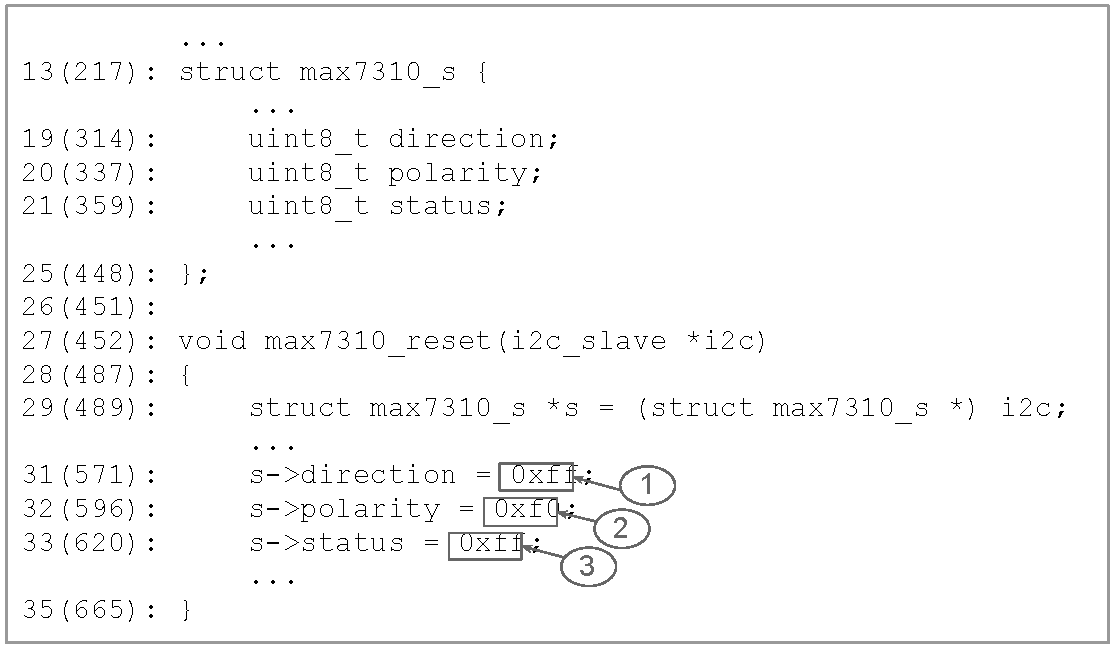
\includegraphics[width=0.95\linewidth]{code1}
\end{minipage}\\
(a) The Old Version\\
\\
\begin{minipage}[b]{\linewidth}
  \centering
  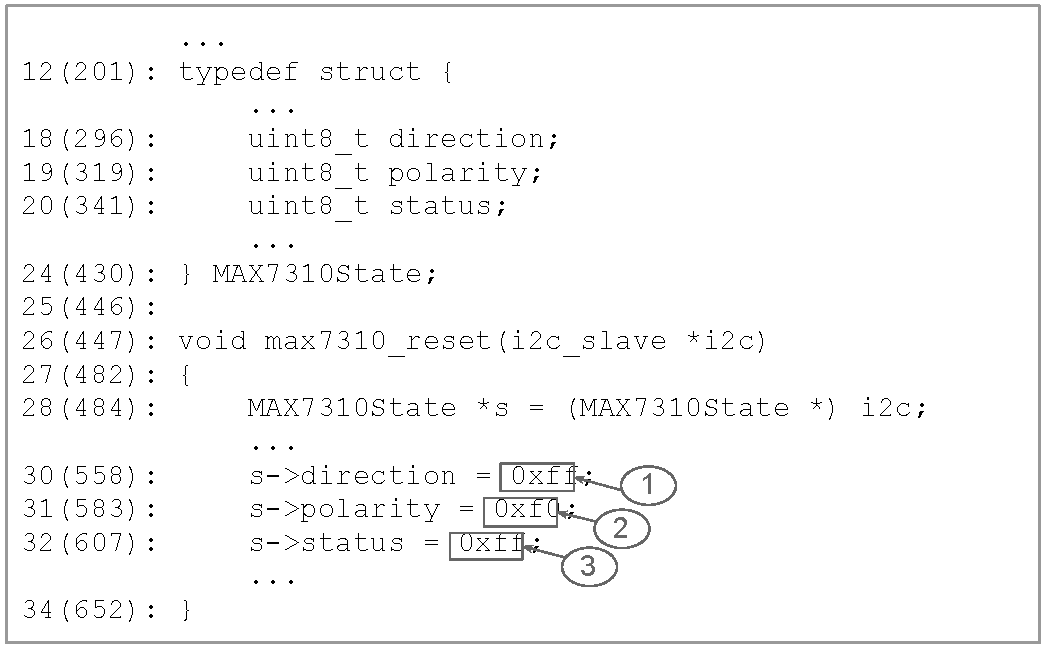
\includegraphics[width=0.95\linewidth]{code2}
\end{minipage}\\
(b) The Newer Version
\end{tabular}
  \caption{Two Versions of a Virtual Devices Written in C. This piece of code is extracted from MAX7310 virtual device in QEMU virtual machine. This code defines a function to reset the registers. However, we do not know why they are resetted to the values labeled 1, 2 and 3. To know the answer, we need to refer to the specification.}
\label{fig:code}
\end{center}
\end{figure}

\begin{figure}
  \centering
  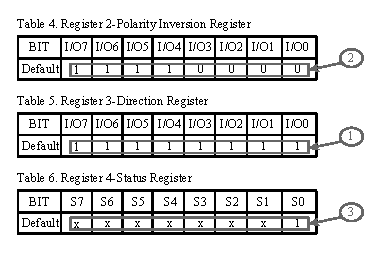
\includegraphics[width=0.7\textwidth]{spec}
  \caption{Specification Example. This is part of MAX7310 specification. It includes three tables, which define the default values for three registers.}
  \label{fig:spec}
\end{figure}

The interfaces between software and hardware are composed of registers exposed by hardware devices and accessible by software. The implementation of the interfaces should conform to the specification in order to function correctly. Suppose we have to maintain and understand this implementation, we need to establish relationships between the implementation and the specification. Fig.~\ref{fig:code}(a) presents part of code extracted from a virtual device prototype for MAX7310 in QEMU. A virtual device prototype is a software implementation emulating a hardware device. MAX7310 is a 8-bit I/O port expander. QEMU (Quick EMUlator)\footnote{\texttt{\url{http://www.qemu.org}}} is virtual machine used widely in industry to assist hardware related software development. The source code for this implementation is written in C language. From the name of the function, we can guess the function shown is trying to reset the device to its initial state. However, we can not figure out what the values in the right sides of the assignment statements mean only by reading the code here. Fig.~\ref{fig:spec} includes the information extracted from the specification of MAX7310. In this figure, we can see three tables for three registers: polarity register, direction register and status register. These tables present the bit arrangement and the default value for each register. By looking at this specification, now we can see that the values used in the code are defined in the specification. The code uses the hex format, and the specification use binary format. The piece of code and the piece of specification labeled with the same number are related, which means the piece of specification explains the piece of code with the same label.

% in the directory including max7310.c: git log --follow --all -p max7310.c > a.txt
Code evolves all the time in its lifecycle. By checking the QEMU repository, we can find that the first version of the code in Fig~\ref{fig:code} was created on May 23, 2007, and the last change is on May 1, 2013. This code has changed 21 times till now, and it still keeps changing. 
Fig.~\ref{fig:code}(b) shows an example of a new version of the code in Fig.~\ref{fig:code}(a). Line 13, 25 and 29 of the code in Fig.~\ref{fig:code}(a) has changed to the line 12, 24 and 28 in Fig.~\ref{fig:code}(b).

Compared to code, specification is relatively stable. The specification in Fig~\ref{fig:spec} only has three versions, and the last change happened in 2005. The specification remains unchanged since the code was created.

This example is simple, but reveals three basic requirements for the management of traceability links between specification and implementations as follows.

\textbf{Requirement 1:} Traciability links should be able to uniquely refer to and accurately locate the relevant pieces of code in the source file and the piece of specification in the specification file. As in the example, there should be a way to locate the code pieces and specification pieces surrounded by the boxes labeled by 1, 2 and 3.

\textbf{Requirement 2:} Traceability links should be able to provide referrence at statement level or expression level for source code and at sentence level or word level for specification. As in this example, the code pieces and specification pieces surrounded by the boxes labeled by 1, 2 and 3 are all on this level.

\textbf{Requirement 3:} Traceability links should be immune from the evolusion of unrelated code. We should grarantee that the identifier created for the old version of code works for the new version of code if the code piece refered by the identifier does not change.

